\documentclass[final]{beamer}
\usepackage{grffile}
\usepackage{ragged2e}
\mode<presentation> {
\usetheme{XDI}
\setbeamercovered{transparent}
}

\usepackage{color,fancybox,alltt,graphicx,listings}
\usepackage{type1cm,calc,times,amsmath,amsthm, amssymb, latexsym}

\boldmath
\usepackage[english]{babel}
\usepackage[latin1]{inputenc}
\definecolor{Red}{rgb}{0.75,0,0}
\definecolor{Blue}{rgb}{0,0,0.75}
\newcommand{\Color}[2]{{\textcolor{#1}{#2}}}

\newcommand{\Red}[1]{{\Color{Red}{#1}}}
\newcommand{\EmphRed}[1]{{\Color{Red}{\emph{#1}}}}
\newcommand{\BoldRed}[1]{{\Color{Red}{\bf{#1}}}}
\newcommand{\Blue}[1]{{\Color{Blue}{\bf{#1}}}}

\usepackage[orientation=portrait,size=a0,scale=1.4]{beamerposter}
\graphicspath{{images/}}

\title[XAFS Data Formats Poster]{Towards Data Format Standardization for X-ray Absorption Spectra}
\author[Newville, Sol\'e, Ravel, and Hester]{
  Matthew Newville${}^{a}$, V. Armando  Sol\'e${}^{b}$,  James R. Hester${}^{c}$, and Bruce Ravel${}^{d}$}
\institute[]{
  ${}^{a}$Center for Advanced Radiation Sources, University of Chicago, USA, \par
  ${}^{b}$European Synchrotron Radiation Facility, Grenoble, France, \par
  ${}^{c}$Bragg Institute, Australian Nuclear Science and Technology Organization, Sydney, Australia, \par
  ${}^{d}$National Institute  of Standards and Technology, Gaithersburg, MD USA
}

  \date{23-July-2012}

  \begin{document}
  \begin{frame}{}

   {\ }   \vspace{-20mm}

    \begin{columns}[t]
      \begin{column}{.01\linewidth}\end{column}

      \begin{column}{.54\linewidth}
        \begin{block}{\large Abstract}
          \justifying

          To facilitate exchange and archiving of X-ray absorption data, we
          propose a data format for $\mu(E)$ or $\chi(k)$ spectra using a
          simple, plain-text file. The XAS Data Interchange (XDI) format
          uses space-delimited columns for numerical absorption data.  As
          such, it is similar to raw data formats currently used at many
          XAS beamlines.  XDI offers a clearly defined structure
          for metadata in the file header.  Several example XDI files and
          programming libraries for reading these files are publicly
          available.  Because XDI accommodates only single spectra, we also
          discuss approaches that are capable of combining multiple XAFS
          spectra and non-XAFS data into multispectral libraries using
          either the hierarchical data format (HDF5) or relational
          databases based either on the CIF format or a SQL-based database
          engine.

        \end{block}

        \begin{block}{\large  X-ray Data Interchange Format:  Exchanging
            XAFS Data}
          \justifying

          The exchange and long term storage of archived XAFS data is a common
          need in the XAFS community.  Retrieving data on
          {\EmphRed{standards}} or {\EmphRed{model compounds}} and using
          data taken at different facilities and beamlines are continuing
          needs for both XANES and EXAFS analysis.

          {\hspace{16mm}} {\Blue{We need to share XAFS spectra between
              facilities for decades to come.}}
          

          \vspace{2mm}

          There is no commonly accepted data format for XAFS data, though
          most data collection and processing software use some form of a
          Plainttext (ASCII) file.  Such files are human-readable and used
          widely in third party applications.

          
        \end{block}
        
        \begin{block}{\large XDI Design Principles}

          \begin{columns}[T]
            \begin{column}{0.05\linewidth}    \end{column}
            \begin{column}{0.90\linewidth}
              
              \begin{enumerate}[I.] \normalsize
              \item $\mu(E)$ and $\chi(k)$ are the spectral ``unit of  currency''
              \item The XDI format should use Plaintext ASCII for maximum portability.
              \item The XDI format should be fully, and publicly documented.
              \item The XDI format must support both array data and meta-data.
              \item The XDI format should be extensible.
              \item Application/programming interfaces (APIs) should be
                available for many computer languages.
              \end{enumerate}

            \end{column}
            \begin{column}{0.05\linewidth}    \end{column}
          \end{columns} 
        \end{block}
        
        \begin{block}{\large XDI: Current Status}

          We currently have, ready for testing:
          \begin{center}
            \begin{minipage}{0.9\linewidth}
              \begin{description}[A]
              \item {\Blue{12 example XDI files}} 12 different spectra, all valid  XDI Files.
              \item {\Blue{C library and Shared Object Library (DLL)}}  for
                reading XDI files:\par   {\hspace{10mm}} Source code, Windows, Mac OSX, Linux binaries.
              \item {\Blue{Python Library}}  Built using C library.
              \item {\Blue{Fortran, Perl Library, Documentation}}  Underway.
                {\BoldRed{Volunteers sought!}}
              \end{description}
            \end{minipage}
          \end{center}
          
        \end{block}
      \end{column}

      \begin{column}{.01\linewidth}
      \end{column}

      \begin{column}{.44\linewidth}
        \begin{block}{Example XDI File}
          \begin{center}
            \begin{minipage}[t]{0.95\linewidth}
              \begin{alltt}
                {\footnotesize
                  \#XDI/1.0  {\BoldRed{$\leftarrow$ Version Info}}\par
                  \#Beamline.name: APS 10ID\par
                  \#Detector.I0:  N2 15cm\par
                  \#Detector.I1:  N2 15cm\par
                  \#Sample.name: gamma-FeO(OH)\par
                  \#Mono.name:  Si 111\par
                  \#Mono.d\_spacing: 3.13553\par
                  \#Element.symbol: Fe\par
                  \#Element.edge: K\par
                  \#Column.1: energy eV
                  {\BoldRed{$\leftarrow$ Column Labels, Units}}\par
                  \#Column.2: mutrans\par
                  \#Column.3: i0\par
                  \#///
                  {\BoldRed{$\leftarrow$ start multi-line comment}}\par
                  \#Fe K-edge, Lepidocrocite powder\par
                  \#on 4 layers of tape\par
                  \#------- {\BoldRed{$\leftarrow$ End Header, Begin Arrays Table}}\par
                  \#\par
                  \hspace{3mm} 6899.9609 -1.3070486 149013.70\par
                  \hspace{3mm} 6900.1421 -1.3006104 144864.70\par
                  \hspace{3mm} 6900.5449 -1.3033816 132978.70\par
                  \hspace{3mm} \ldots\par
                }
              \end{alltt}
            \end{minipage}
          \end{center}
        \end{block}

        \vspace{2mm}
        \begin{block}{\large XDI File description}

          \justifying
          Some metadata are \textbf{required} in all files (case insensitive):

         \begin{center}
           \begin{minipage}[t]{0.95\linewidth}
             \begin{description}[Mono]
             \item[\Blue{Element.symbol}]  Atomic symbol of absorbing element
             \item[\Blue{Element.edge}]    K, L3, M4, etc
             \item[\Blue{Mono.d\_spacing}]  Required if mono angle is given and mono energy is not.
               Strongly encouraged for all data,
             \end{description}
           \end{minipage}
         \end{center}

         \vspace{3mm}

          \hrule

          \vspace{3mm} {\ }

          Supported column labels.

         \begin{columns}[T]
           \begin{column}{0.06\linewidth}
           \end{column}
           \begin{column}{0.41\linewidth}
             \begin{itemize}
             \item {\Blue{\tt{energy}}}  Mono Energy, in eV or keV.
             \item {\Blue{\tt{angle}}}   Mono Angle, in degrees.
             \item {\Blue{\tt{i0}}}      Monitor, $I_0$.
             \item {\Blue{\tt{time}}}    Integration time.
             \item {\Blue{\tt{itrans}}}  Transmitted intensity, $I_1$.
             \item {\Blue{\tt{ifluor}}}  Fluorescence intensity, $I_f$.
             \item {\Blue{\tt{irefer}}}  Reference signal, $I_2$.
             \end{itemize}
           \end{column}
           \begin{column}{0.06\linewidth}
           \end{column}
           \begin{column}{0.41\linewidth}
               \begin{itemize}
               \item {\Blue{\tt{mutrans}}}   $\mu(E) = -\ln(I_1/I_0)$.
               \item {\Blue{\tt{mufluor}}}   $\mu_f(E) = I_f/I_0$
               \item {\Blue{\tt{murefer}}}   $\mu_r(E) = -\ln(I_2/I_1)$.
               \item {\Blue{\tt{normtrans}}} Normalized $\mu(E)$
               \item {\Blue{\tt{normfluor}}} Normalized $\mu_f(E)$
               \item {\Blue{\tt{normrefer}}} Normalized $\mu_r(E)$
               \item {\Blue{\tt{k}}}         Wavenumber
               \item {\Blue{\tt{chi}}}       $\chi(k)$
               \end{itemize}
           \end{column}
           \begin{column}{0.06\linewidth}
           \end{column}
         \end{columns}

         \vspace{3mm}

         \hrule

         \vspace{3mm} {\ }

         \justifying
         Other metadata describe additional information about the spectra, with
         entries arranged as {\BoldRed{{Family.Keyword: Value}}}.  Families include:

         \begin{columns}[T]
           \begin{column}{0.02\linewidth}
           \end{column}
           \begin{column}{0.46\linewidth}
             \begin{itemize}
             \item {\Blue{\tt{Column}}}   labels for array columns
             \item {\Blue{\tt{Element}}}  absorbing element (edge)
             \item {\Blue{\tt{Mono}}}     monochromator (d-spacing)
             \item {\Blue{\tt{Facility}}} facility  (name, x-ray source)
           \end{itemize}
           \end{column}
           \begin{column}{0.02\linewidth}
           \end{column}
           \begin{column}{0.46\linewidth}
             \begin{itemize}
             \item {\Blue{\tt{Beamline}}} beamline  (name, optics)
             \item {\Blue{\tt{Scan}}}     scan  (step size, date)
             \item {\Blue{\tt{Detector}}} detector (types, gases)
             \item {\Blue{\tt{Sample}}}   sample (name, prep)
           \end{itemize}

           \end{column}
           \begin{column}{0.02\linewidth}
           \end{column}

         \end{columns}

         \hspace{3mm}

         This list is not exhaustive.  XDI is extensible, and new metadata
         fields can be added without affecting other applications.


       \end{block}
     \end{column}

   \end{columns}

   % \begin{columns}[T]
   %   \begin{column}{.01\linewidth}\end{column}
   %   \begin{column}{.98\linewidth}     
   
   \begin{block}{\large Storing and Managing Multiple XDI Spectra:  Data Libraries}
     
     An XDI file contains exactly one $\mu(E)$ or $\chi(k)$ XAFS
     spectrum.  To support libraries of spectra or multi-spectral data
     sets, we propose three possible solutions to complement XDI for multiple spectra.
     These suggestions should not be viewed as exclusive.
         
     \vspace{-3mm}
     
   \end{block}
   

   {\ }   \vspace{-20mm}


%      \end{column}
%      \begin{column}{.01\linewidth}\end{column}
%    \end{columns}
% 

    \begin{columns}[t]
      \begin{column}{.01\linewidth}\end{column}
      \begin{column}{.31\linewidth}
        \begin{block}{HDF5 -- Hierarchical Data Format}

          \justifying Multiple Spectra held hierarchically, with highly
          optimized data arrays.  HDF5 is becoming standard at synchrotrons
          for very large datasets.  Excellent library support.

         \vspace{6mm}

         \begin{center}
           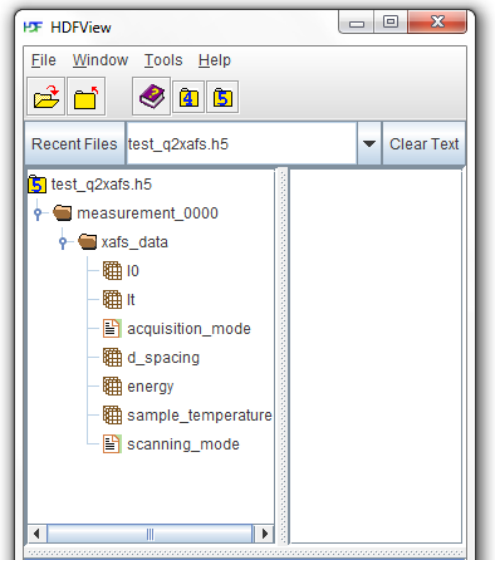
\includegraphics[width=0.62\linewidth]{hdf5.png}
         \end{center}

         \vspace{10mm} {\ }   \vspace{10mm} {\ }

        \end{block}
      \end{column}
      \begin{column}{.01\linewidth}
      \end{column}
      \begin{column}{.34\linewidth}
        \begin{block}{Crystallographic Information Framework}

          \justifying CIF can encapsulate one or more data sets in a text
          file.  Within each block, data and meta-data appear as key-value
          pairs or in a series of tables.  This gives a text representation
          of a relational database.

          \begin{center} \begin{minipage}{0.66\linewidth}
              \begin{alltt}
                {\tiny
                  data\_v2o5\_nanotube\par
                  \_xafs\_absorber.atom   V\par
                  \_xafs\_absorber.edge    K\par
                  \_xafs\_source.identification   'KEK-PF BL20B'\par
                  \_xafs\_source.location         'Tsukuba, Japan'\par
                  loop\_\par
                  \_xafs\_detectors.label xafs\_detectors.position
                  \_xafs\_detectors.type\par
                  monitor      monitor    ionisation\par
                  io-detector  detector   ionisation    foil         foil       ionisation\par
                  \par
                  loop\_\par
                  \_xafs\_ionisation\_detector.label\par
                  \_xafs\_ionisation\_detector.gas\_pressure\par
                  \_xafs\_ionisation\_detector.length\par
                  \_xafs\_ionisation\_detector.amplifier\_type\par
                  \_xafs\_ionisation\_detector.amplifier\_gain\par
                  monitor         1      10    'Keithley'    10\par
                  io-detector     1      20    'Keithley'    10\par
                  foil            1      5     'Keithley'    11\par
                  \par
                  loop\_\par
                  \_xafs\_reduced.energy \_xafs\_reduced.absorbance\par
                  5248.52108 0.813707373\par
                  5258.29435 0.798733337\par
                  5268.26606 0.781069442\par
                  \ldots\par
                }
              \end{alltt}
              \end{minipage} \end{center}


         \vspace{10mm} {\ }  \vspace{10mm} {\ }

        \end{block}
      \end{column}
      \begin{column}{.01\linewidth}
      \end{column}
      \begin{column}{.31\linewidth}
        \begin{block}{SQLite -- relational database in a file}

          \justifying A true relational database in a portable file. Supports
          SQL and many languages.  An industry standard for
          data storage. Like ASCII, not high performance for numerical
          arrays.

         \vspace{6mm}

         \begin{center}
           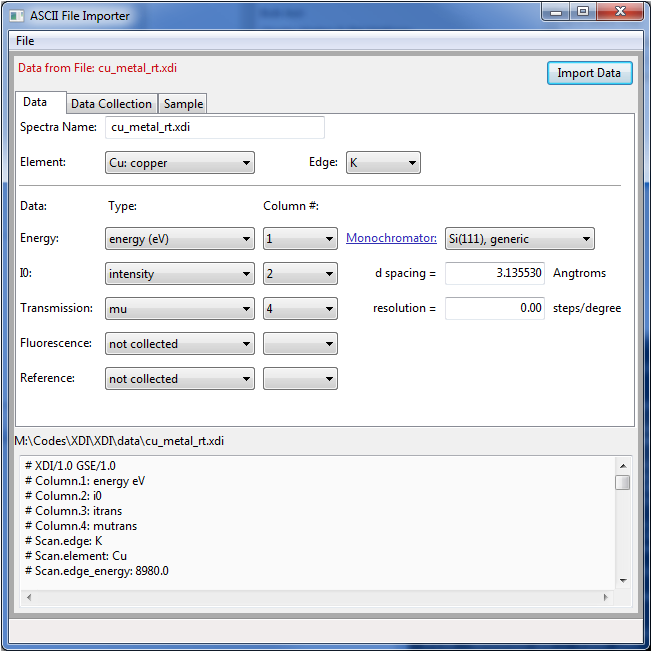
\includegraphics[width=0.7\linewidth]{sqlite.png}
         \end{center}

         \vspace{10mm} {\ }   \vspace{10mm} {\ }


        \end{block}
      \end{column}
      \begin{column}{.01\linewidth}
      \end{column}

    \end{columns}
  \end{frame}
\end{document}
